\chapter{Исследовательская часть}

В данном разделе будут приведены примеры работы программы, и проведены замеры процессорного времени и предоставлена информация о технических характеристиках устройства..

\section{Технические характеристики}

Ниже представлены характеристики компьютера, на котором проводились замеры времени  работы реализации алгоритмов:

\begin{itemize}
	\item операционная система Windows 10 Домашняя 21H2;
	\item оперативная память 12 Гб;
	\item процессор Intel(R) Core(TM) i7-9750H CPU @ 2.6Гц.
\end{itemize}

Загруженность компонентов:

\begin{itemize}
	\item процессор - 10\%;
	\item оперативная память - 53\%
\end{itemize}

\clearpage

\section{Демонстрация работы программы}

На рисунке \ref{img:example}-\ref{img:example2} приведен пример работы программы.

\begin{figure}[H]
	\begin{center}
		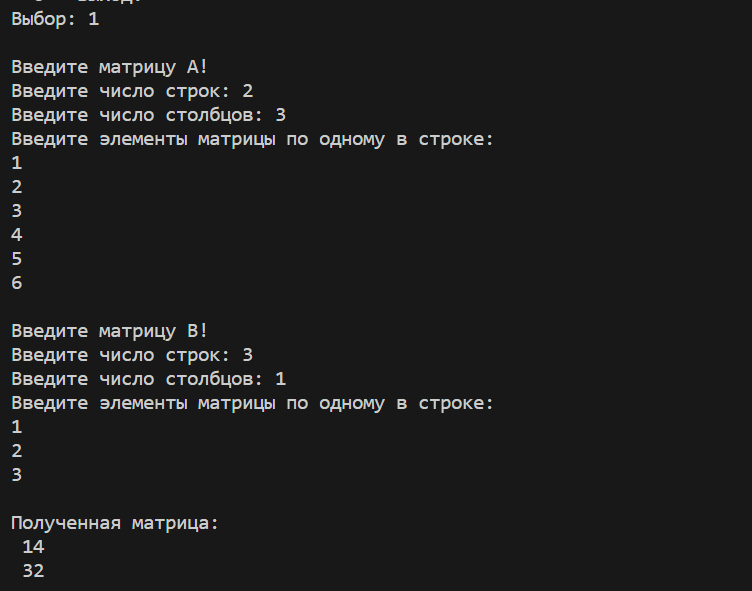
\includegraphics[scale=0.8]{img/example.png}
	\end{center}
	\captionsetup{justification=centering}
	\caption{Пример работы стандарного алгоритма}
	\label{img:example}
\end{figure}
\begin{figure}[H]
	\begin{center}
		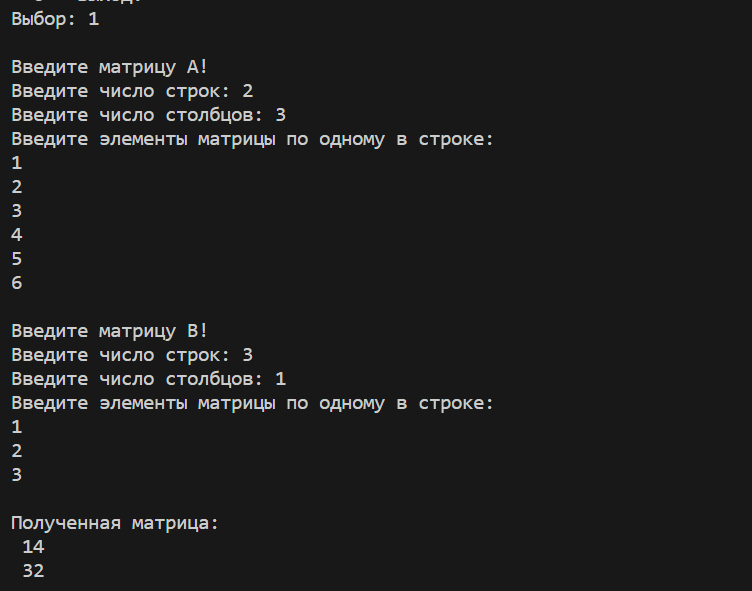
\includegraphics[scale=0.8]{img/example.png}
	\end{center}
	\captionsetup{justification=centering}
	\caption{Пример работы алгоритма Винограда}
	\label{img:example1}
\end{figure}
\begin{figure}[H]
	\begin{center}
		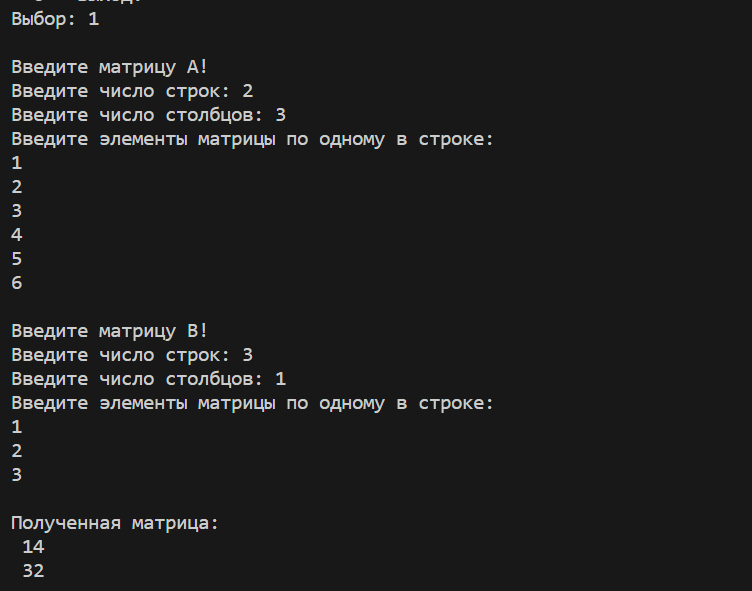
\includegraphics[scale=0.8]{img/example.png}
	\end{center}
	\captionsetup{justification=centering}
	\caption{Пример работы алгоритма Штрассена}
	\label{img:example2}
\end{figure}

\section{Время выполнения алгоритмов}

Функция process\_time из библиотеки time ЯП Python возвращает  процессорное время в секундах - значение типа float.

Для замера времени:
\begin{itemize}
	\item получить значение времени до начала выполнения алгоритма, затем после её окончания. Чтобы получить результат, необходимо вычесть из второго значения первое;
	\item первый шаг необходимо повторить iters раз (в программе iters равно 100), суммируя полученные значения, а затем усреднить результат.
\end{itemize}

Замеры проводились для квадратных матриц целых чисел, заполненных случайным образом, размером от 10 до 100 и от 11 до 101. Результаты измерения времени для четного размера матриц приведены в таблице \ref{tbl:time_even} (в мс).

\begin{table}[h]
    \begin{center}
        \begin{threeparttable}
        \captionsetup{justification=raggedright,singlelinecheck=off}
        \caption{Результаты замеров времени}
        \label{tbl:time_even}
        \begin{tabular}{|c|c|c|c|c|}
        	\hline
        	& \multicolumn{4}{c|}{\bfseries Выходные данные по алгоритму} \\\cline{2-5}
        	Размер & Стандартный & Винограда & Опт-ый Винограда & Штрассена  
        	\csvreader{time_even.csv}{}
        	{\\\hline\csvcoli & \csvcolii & \csvcoliii & \csvcoliv & \csvcolv } \\
        	\hline
        \end{tabular}
    \end{threeparttable}
\end{center}
\end{table}

На рисунке \ref{img:graph_even1} - \ref{img:graph_even2} приведены графические результаты сравнения временных характеристик для четного размера матриц.

\begin{figure}[H]
	\begin{center}
		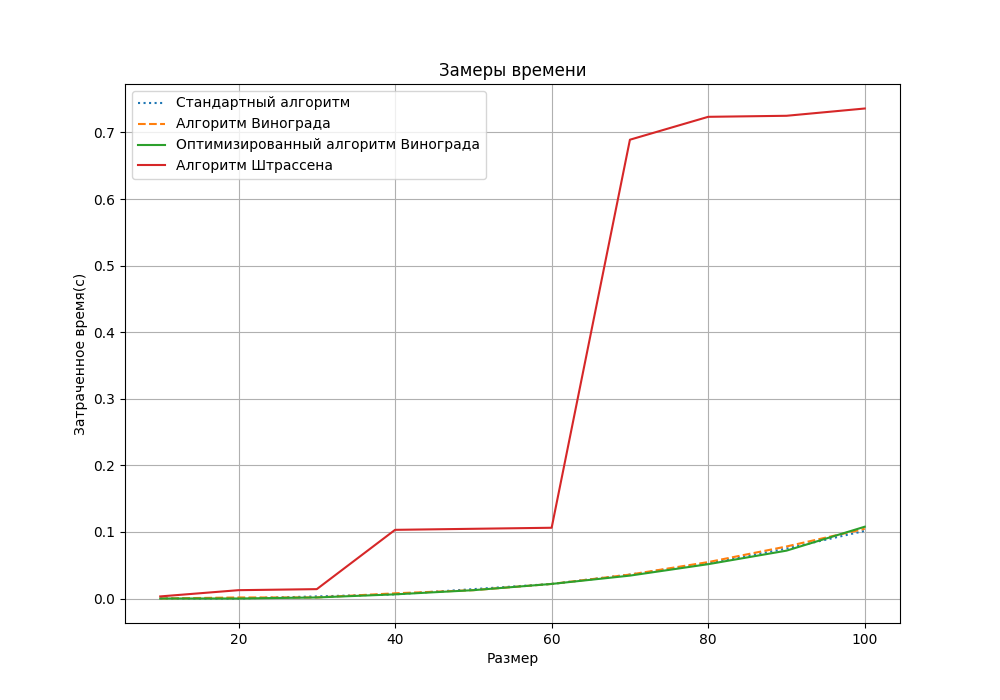
\includegraphics[scale=0.6]{img/graph_even1.png}
	\end{center}
	\captionsetup{justification=centering}
	\caption{Сравнение по времени алгоритмов умножения матриц четного размера}
	\label{img:graph_even1}
\end{figure}

\begin{figure}[H]
	\begin{center}
		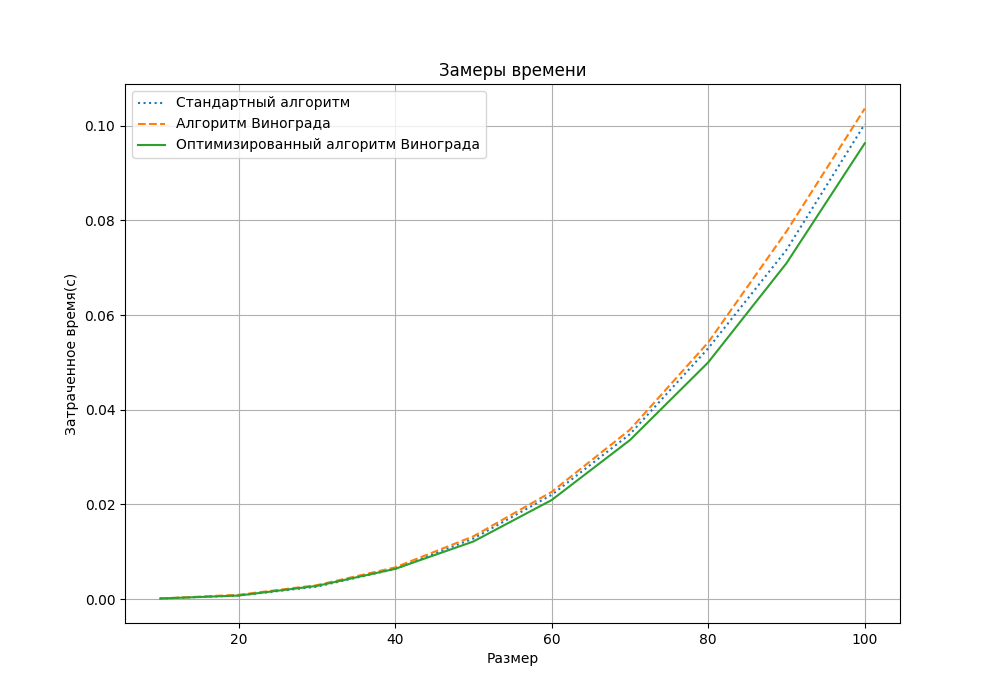
\includegraphics[scale=0.6]{img/graph_even2.png}
	\end{center}
	\captionsetup{justification=centering}
	\caption{Сравнение по времени алгоритмов умножения матриц четного размера}
	\label{img:graph_even2}
\end{figure}

Результаты измерения времени для четного размера матриц приведены в таблице \ref{tbl:time_odd} (в мс).

\begin{table}[h]
    \begin{center}
        \begin{threeparttable}
        \captionsetup{justification=raggedright,singlelinecheck=off}
        \caption{Результаты замеров времени}
        \label{tbl:time_odd}
        \begin{tabular}{|c|c|c|c|c|}
        	\hline
        	& \multicolumn{4}{c|}{\bfseries Выходные данные по алгоритму} \\\cline{2-5}
            Размер & Стандартный & Винограда & Опт-ый Винограда & Штрассена
			\csvreader{time_odd.csv}{}
			{\\\hline\csvcoli & \csvcolii & \csvcoliii & \csvcoliv & \csvcolv } \\
			\hline
		\end{tabular}
    \end{threeparttable}
\end{center}
\end{table}

На рисунке \ref{img:graph_odd1}-\ref{img:graph_odd2} приведены графические результаты сравнения временных характеристик для нечетного размера матриц.

\begin{figure}[H]
	\begin{center}
		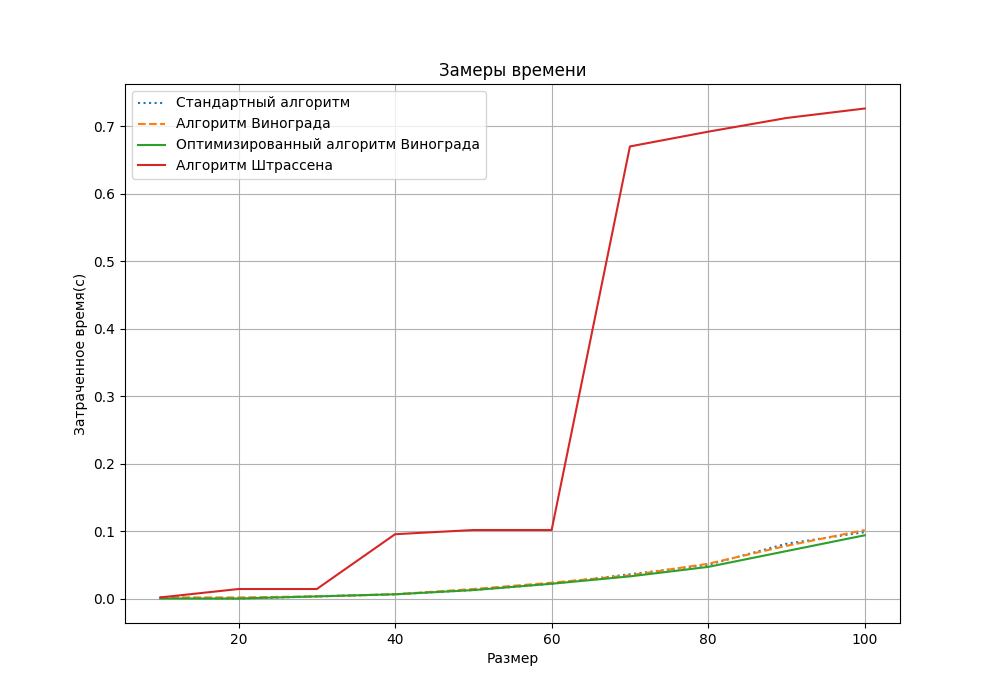
\includegraphics[scale=0.6]{img/graph_odd1.png}
	\end{center}
	\captionsetup{justification=centering}
	\caption{Сравнение по времени алгоритмов умножения матриц нечетного размера}
	\label{img:graph_odd1}
\end{figure}

\begin{figure}[H]
	\begin{center}
		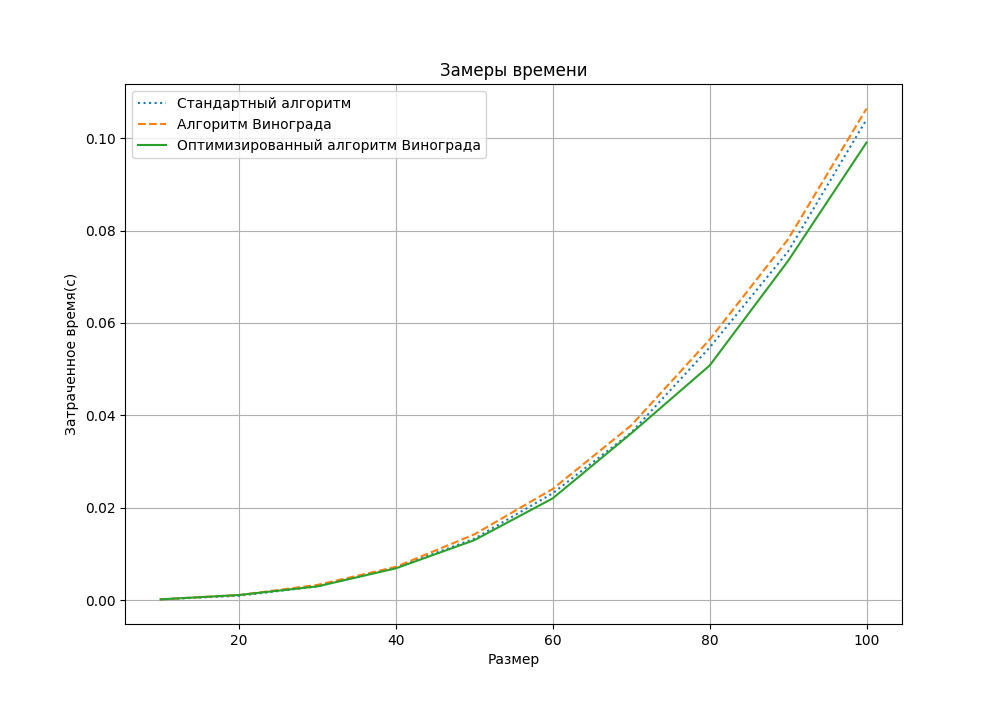
\includegraphics[scale=0.6]{img/graph_odd2.png}
	\end{center}
	\captionsetup{justification=centering}
	\caption{Сравнение по времени алгоритмов умножения матриц нечетного размера}
	\label{img:graph_odd2}
\end{figure}

\section{Использование памяти}

Затраты по памяти для реализации стандарного алгоритма умножения матриц:
\begin{itemize}
	\item матрица A: $n \cdot p \cdot \text{sizeof}(\text{int})$;
	\item матрица B: $p \cdot m \cdot \text{sizeof}(\text{int})$;
	\item результирующая матрица: $n \cdot m \cdot \text{sizeof}(\text{int})$;
	\item размер матриц n, m, p: $3\cdot \text{sizeof}(\text{int})$;
	\item дополнительные переменные (i, j, k): $3\cdot \text{sizeof}(\text{int})$;
	\item адрес возврата.
\end{itemize}

Итого:
\begin{equation}
	\label{eq:stand_alg}
	(n \cdot p + p \cdot m + n \cdot m + 6) \cdot \text{sizeof}(\text{int})
\end{equation}

Затраты по памяти для реализации алгоритма Винограда умножения матриц:
\begin{itemize}
	\item матрица A: $n \cdot p \cdot \text{sizeof}(\text{int})$;
	\item матрица B: $p \cdot m \cdot \text{sizeof}(\text{int})$;
	\item результирующая матрица: $n \cdot m \cdot \text{sizeof}(\text{int})$;
	\item размер матриц n, m, p: $3\cdot \text{sizeof}(\text{int})$;
	\item дополнительные переменные (i, j, k): $3\cdot \text{sizeof}(\text{int})$;
	\item дополнительные массивы row\_factors, column\_factors: $(n + m) \cdot\text{sizeof}(\text{int})$;
	\item адрес возврата.
\end{itemize}

Итого:
\begin{equation}
	\label{eq:wino_alg}
	(n \cdot p + p \cdot m + n \cdot m + 6 + (m + n)) \cdot \text{sizeof}(\text{int})
\end{equation}


Затраты по памяти для реализации оптимизированного алгоритма Винограда умножения матриц:
\begin{itemize}
	\item матрица A: $n \cdot p \cdot \text{sizeof}(\text{int})$;
	\item матрица B: $p \cdot m \cdot \text{sizeof}(\text{int})$;
	\item результирующая матрица: $n \cdot m \cdot \text{sizeof}(\text{int})$;
	\item размер матриц n, m, p: $3\cdot \text{sizeof}(\text{int})$;
	\item дополнительные переменные (i, j, k, row\_factors\_temp, temp\_Ai, index): $5\cdot \text{sizeof}(\text{int})$;
	\item дополнительные переменные row\_factors, column\_factors: $(n + m) \cdot\text{sizeof}(\text{int})$;
	\item адрес возврата.
\end{itemize}

Итого:
\begin{equation}
	\label{eq:optimized_alg}
	(n \cdot p + p \cdot m + n \cdot m + 8 + m + n) \cdot \text{sizeof}(\text{int})
\end{equation}

Затраты по памяти для реализации алгоритма Штрассена умножения матриц. Для работы алгоритма то матрица должен быть квадратная и размер в виде $n = 2^k$:
\begin{itemize}
	\item матрица A: $n \cdot n \cdot \text{sizeof}(\text{int})$;
	\item матрица B: $n \cdot n \cdot \text{sizeof}(\text{int})$;
	\item результирующая матрица: $n \cdot n \cdot \text{sizeof}(\text{int})$;
	\item размер матриц n, m, p: $3\cdot \text{sizeof}(\text{int})$;
	\item дополнительные переменные: $1\cdot \text{sizeof}(\text{int})$;
	\item дополнительные матрицы a, b, c, d, e, f, g, h, p1, p2, p3, p4, p5, p6, p7, c11, c12, c21, c22: $19 * \dfrac{n \cdot m }{{h}^2} \cdot\text{sizeof}(\text{int})$;
	\item адрес возврата.
\end{itemize}

K - количество вызовов рекурсии:

\begin{equation}
	K = log_2(N)
\end{equation}

h - 4 * глубина рекурсии

\begin{equation}
	h = 4 * k (1<= k <= K)
\end{equation}

Итого:
\begin{equation}
	\label{eq:strassen}
	(3 \cdot n \cdot n + 4 + 19 * \dfrac{n \cdot n }{{h}^2}) \cdot \text{sizeof}(\text{int})
\end{equation}


На рисунках \ref{img:mem} также приведены результаты замеров памяти. 

\begin{figure}[H]
	\begin{center}
		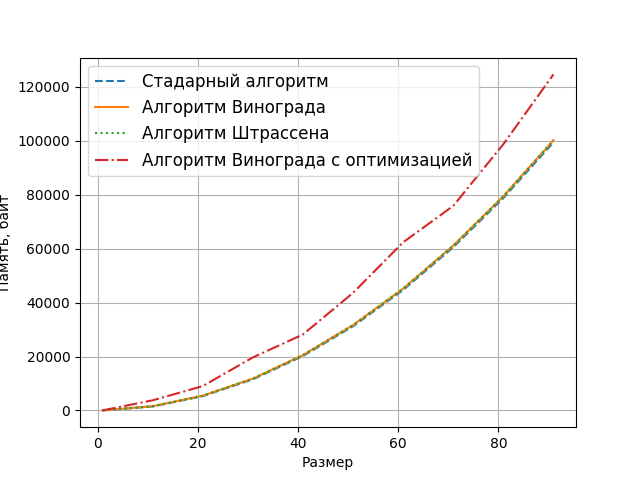
\includegraphics[scale=0.7]{img/mem.png}
	\end{center}
	\captionsetup{justification=centering}
	\caption{Замеры памяти, которую затрачивают реализации алогритмов}
	\label{img:mem}
\end{figure}
\section{Вывод}

В результате эксперимента было получено, что при размере матриц большем 50, оптимизированный алгоритм Винограда работает работает быстрее стандартного алгоритма в 1.1 раза. При этом стандартный алгоритм бытсрее алгоритма Винограда в 1.25 раза. Алгоритм Штрассена работает медленее останых хотя при размере матриц большее 50 уже работает медленее 7 раза. Тогда, для размера матриц, начиная с 50 элементов, небходимо использовать оптимизированный алгоритм умножения матриц по Винограду.

Также в результате эксперимента было установлено, что при четном размере матриц, алгоритм Винограда работает быстрее, чем на матрицах с нечетным размером в 1.2 раза в связи с проведением дополнительных вычислений для крайних строк и столбцов. Можно сделать вывод, что алгоритм Винограда предпочтительно использовать для умножения матриц четных размеров.